In this chapter we provide an overview of our work on scaling boosted tree
learning. We tackle the problem in two different domains: online boosting
(\boostvht) and batch gradient boosting (\blockgbt). We develop algorithms
that are optimized for the distributed setting by being communication efficient
and exhibiting good scaling characteristics.

\section{Background}
\label{sec:scalable-boosted-background}

% Describe the problem
Boosting algorithms are some of the most successful and widely used algorithms
in machine learning, due to their simplicity and excellent accuracy. As a result,
a wide array of research has been proposed with the aim of improving the scalability
of boosting, either through parallelizing the base algorithm, or by developing
algorithms that can perform boosting online.

% Previous approaches and why they don't work
However, when it comes to high dimensional data, current approaches fall short
in terms of scalability.
In the online domain, due to the sequential nature of online boosting algorithms,
current online methods do not make use of parallelism for training~\cite{online-gradient-boosting, Oza2001online, online-boosting-theoretical}.
On the other hand, existing methods for the batch
domain provide parallelism along only the data point dimension, limiting their
scale-out capabilities. As a result, for high-dimensional data with millions
of features, we are left with few choices: In the online domain there exist
no parallel algorithms, while in the batch domain the existing feature-parallel
algorithms make the assumption that the entire dataset can fit in the memory
of each worker, severely limiting the size of the problems we can tackle
\cite{lightgbm, xgboost}.

% Our method
In our work we tackle each domain separately:
In \boostvht, we enable parallelism in the online learning setting, while maintaining the guarantees of existing
online boosting algorithms. To achieve that, we use a sequential ensemble of model-parallel learners that train
on different parts of a single data point in a distributed environment.
In the batch domain we enable scalability across \emph{both} the data point and
feature dimensions by developing a block-distributed gradient boosted tree algorithm.
We show how to make block-distributed training feasible and communication-efficient.

\section{Online and Distributed Boosted Trees}
\label{sec:boostvht-method}

In \boostvht we make parallel online boosting possible, while maintaining the
correctness of the online boosting algorithms, by using model-parallel learning
instead of the data-parallel approaches used in the batch setting.
We make use of the Vertical Hoeffding Tree (VHT) algorithm \cite{kourtellis2016vht} which is a model-parallel
extension of the online Hoeffding tree algorithm \cite{vfdt}, often referred to as
Very Fast Decision Tree (VFDT).
We call our algorithm BoostVHT.

We provided a description of the VFDT algorithm in Section \ref{sec:bg-dt-online-trees}.
Briefly, the VFDT algorithm will sort instances down the tree and update the statistics for the
leaf the instance ends up in. This separation of duties allows for the scalable design of
VHT: the algorithm uses two components, one called the \emph{model aggregator}
that is responsible for sorting instances to leafs and maintaining the model, and
one called the \emph{local statistics}, which are potentially many workers responsible
for maintaining the statistics for the leaves of the tree.
The model aggregator is responsible for breaking up each instance into its constituent
features, and sending them, along with the label, to the local statistics workers.
The model aggregator will periodically query the local statistics to check if we have
collected enough information to split each leaf with high confidence, as done in the
original VFDT.

\subsection*{Optimizations}

Our method proposes optimizations that make the learning process efficient in a distributed
setting. We use a design that is similar to the original VHT in that we maintain
two main components, one model aggregator and local statistics. However, our model
aggregator hosts a sequential chain of VHT models, through which we pass each example.
This design allows us to maintain the sequential nature of the boosting algorithm,
and as a result the guarantees of any online boosting algorithm, while performing
the training in parallel and asynchronously in a set of local statistics workers.

We propose three optimizations over the original VHT algorithm to improve its
characteristics for distributed boosting. First, we design our local statistics
so that the same worker can host statistics from multiple members of the ensemble.
This enables to decouple the level of parallelism from the number of learners
in the ensemble, separating the algorithm's functional (speedup) and non-functional
(accuracy) aspects.
Second, this enables us to host the statistics for a range of features on the same
worker, across the ensemble. This makes our communication pattern efficient:
We only need to send $p$  messages per instance, where $p$ is the chosen
parallelism level, compared to sending $m$ messages, where $m$ the
number of features. This will dramatically
reduce the number of messages sent, since $m \gg p$ in the high-dimensional
settings we are focusing on. In addition, compared to existing
parallel boosting methods like AdaBoost.PL \cite{adaboost-pl} that needs to communicate the complete
models between each update, we only need to communicate the split decisions which are
much more compact (3 floating point values instead of a complete tree data structure).
Finally, our approach allows us to send each attribute slice only once to
each worker, as it suffices for each subsequent learner after the first
to only send their updated weight. This brings a communication reduction
of a factor $s$, where $s$ is the ensemble size, which can often be hundreds of
trees~\cite{hundreds-classifiers}.

\section{Block-distributed Gradient Boosted Trees}
\label{sec:block-gbt}

In \blockgbt we extend distributed gradient boosted trees, by parallelizing their
training across both the data point and feature dimensions, making use of block-distribution.
Here we provide a summary of each part of the training algorithm that we had to
adapt to the block-distributed setting. We provided an explanation of the training
process for GBTs in Section \ref{sec:bg-dt-gbts}, and we briefly re-iterate here:
The training process can be roughly divided into three stages: First comes
the prediction part, in which we use the existing ensemble to make a prediction
for each point in the dataset. We use these predictions to get the gradient
value for each data point. Second comes the gradient histogram creation.
In this stage we use the computed gradients to create gradient histograms
for every feature, one for each leaf in the tree. A gradient histogram
for a feature contains in each bucket the sum of the gradients that corresponds to
that feature range. Finally, given the gradient histograms for each feature,
we have a final step of split selection, where we use these histograms to greedily
select the optimal split for each leaf.

\subsection{Block-distributed prediction}
\label{subsec:block-gbt-prediction}

In the row-distributed setting, each worker has access to all the features for the
horizontal slice of the data they are responsible for. This allows us to determine
the exit node for each local data point without any communication.
That is not the case however
for block-distributed data where each worker only has access to parts of each data
point. In this case, when the model contains internal nodes that correspond to features
that are not present in one worker, they will need to communicate with the other
workers responsible for the same horizontal slice to determine the exit nodes.
What we want to avoid in this scenario is shuffling the data between workers,
as we could have millions of features leading to impractical communication
costs. In our approach we develop a novel use of the Quickscorer \cite{quickscorer} algorithm
that gives us provably correct and efficient block-distributed predictions.

Briefly, in Quickscorer the exit node for a data point dropped down a decision tree can be determined by applying the bit-wise
\AND operation between specific bit-strings for every internal node.
These bit-strings are of length $|L|$, where $L$ the set of leaves, and
every zero indicates that a leaf node becomes impossible to reach if the node's
condition evaluates to false, and all other elements are one. When determining
the exit node for a particular example, we need to identify all the nodes in
the tree that evaluate to false for that example, and aggregate their bit-strings into one overall
bit-string \bitstring.
\citet{quickscorer}
prove that the left-most bit set to one in \bitstring will indicate the exit node for the example.

We provide an illustrative example, re-using the data from Section \ref{sec:bg-dt-gbts},
which we reproduce in Table \ref{tab:example-data-reprod}. An example decision tree
is given in Figure \ref{fig:quickscorer-example}, along with the corresponding
bit-strings for each internal node. Each bit in the bit-string
corresponds to one of the leafs of the tree, with the left-most bit corresponding
to the left-most leaf. For example, the bit-string for the root is $0011$, because
if the root evaluates to false, the two left-most leaves become inaccessible
(we move right when a node evaluates to false), but either of the
two right-most leaves could still be reached.

Let's take data point 2, which has the feature values $f1: 7, f2:1 , f3: 667$.
Using our oracle we can tell that the nodes that evaluate to false are the root, as $7 > 5$,
and its right child, as $667 > 500$. Their bit-strings are $0011$ and $1101$ respectively. To determine
the exit node we simply need to perform an \texttt{AND} operation between these two
bit-strings: $0011 \land 1101 = 0001$. The left-most bit set to one
is bit 4 (or 3 if we are using 0-indexing), hence the exit node corresponds
to the fourth leaf from the left. We can verify that is true by following the tree
conditions.

\begin{table}
	\centering
	\begin{tabular}{cccc|c}
		\toprule
		Index & Feature 1 & Feature 2 & Feature 3 & Gradient \\
		\midrule
		\rowcolor{CBOne}
		1 & 13 & 0 & 488 & 1.5 \\
		\rowcolor{CBTwo}
		2 & 7 & 1 & 667 & 2.5 \\
		\rowcolor{CBThree}
		3 & 3.5 & 0 & 122 & 2 \\
		\rowcolor{CBFour}
		4 & 1.6 & 2 & 366 & 2.5 \\
		\bottomrule
	\end{tabular}
	\caption{Example dataset.}
	\label{tab:example-data-reprod}
\end{table}

\begin{figure*}
	\centering
	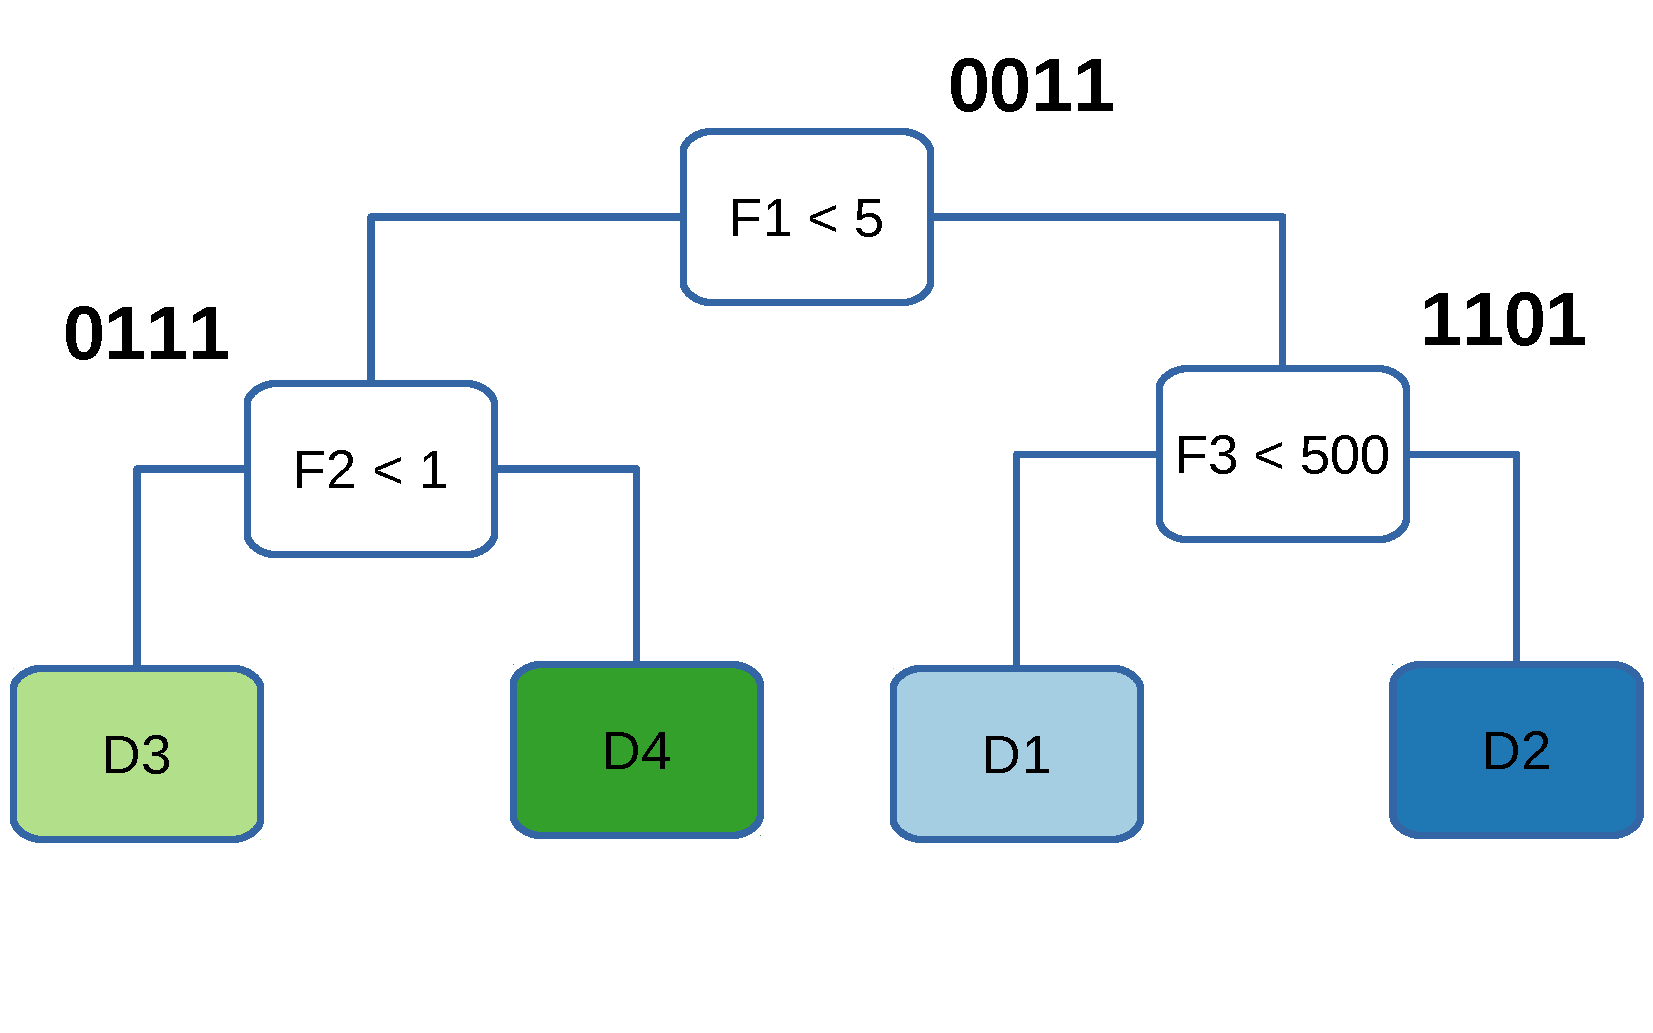
\includegraphics[width=0.8\textwidth]{decision_tree}
	\caption{Example decision tree, and the end positions of the data points in Table
	\ref{tab:example-data-reprod}. When a node condition evaluates to false, we move to
	the right child of the node.
	The bitstring  zeros indicate the leafs that become unreachable when a node evaluates to false.}
	\label{fig:quickscorer-example}
\end{figure*}


We adapt the above algorithm to work in the block-distributed setting. Each worker
now only has access to particular range of features for a subset of the data points.
So each worker can only evaluate the conditions of the tree that correspond to its slice
of the features. We create local bit-strings at each worker, one for each example.
These bit-strings have the same properties as in the original Quikscorer algorithm,
however can only eliminate leafs that are children of internal nodes that correspond
to the features available at that worker. To fully determine the output for each
data point, the workers that hold data for the same horizontal slice will need
to aggregate their bit-strings for each data point. We do this by utilizing the
parameter server \cite{muPS} architecture: Each server is responsible for a
one horizontal slice of the data. The workers that hold the different parts of
a horizontal slice, all send their local bit-strings to the same server, for each example in
their data block.
The server then aggregates the partial bit-strings using a simple bit-wise \AND to determine the exit
node for each data point.

In our example, say data point 2 was split between two workers, Worker 1 and Worker 2,
with Worker 1 responsible for Features 1 \& 2, and Worker 2 responsible for Feature 3.
Worker 1 would be able to only evaluate the condition of the root as false and produce
the local bistring $0011$ and Worker 2 would evaluate the condition involving Feature 3, producing
the local bistring $1101$. Each worker sends their local bit-strings to the same server,
where they are aggregated to produce the final bit-string $0001$.

Because the \AND operator is both commutative and associative, the order in which
these aggregations happen does not affect the result, and the overall aggregation
will be equal to the aggregation of the partial aggregations. This ensures that
our predictions will be correct. By using this method we can determine the exit
nodes for each data point, and from that, the corresponding gradients that we need
for the next step of histogram aggregation. By only communicating bit-strings
and performing bitwise operations that are hardware optimized we ensure that
the communication and computation cost of this step remains low.

\subsection{Histogram Aggregation}
\label{subsec:block-gbt-histogram-aggregation}


With centralized data the histogram aggregation step requires no communication,
and can be performed by running a simple local aggregation.
In the example given in Section \ref{sec:bg-dt-gbts}, we determined the full
gradient histograms for all features and data points by aggregating the
gradient values for each feature range bucket.
In that example we had three buckets per feature, determined by the empirical
CDF of each feature, which we populated by iterating through each feature
value in the current leaf partition. The resulting full histogram was
shown in Figure \ref{fig:gradient-all-features}. We  again use the
data from Table \ref{tab:example-data-reprod}.


Now assume that we have a row-distributed dataset, where we assign data points 1 and 2 to Worker 1, and data points 3 and 4 to
Worker 2.
To get a complete picture of the gradient histograms as shown in Figure \ref{fig:gradient-all-features}, we need to first create local histograms at each worker, and
then aggregate them between the workers, meaning that the the algorithm involves one communication
step.

\begin{figure}
	\centering
	\begin{subfigure}[t]{\textwidth}
		\centering
		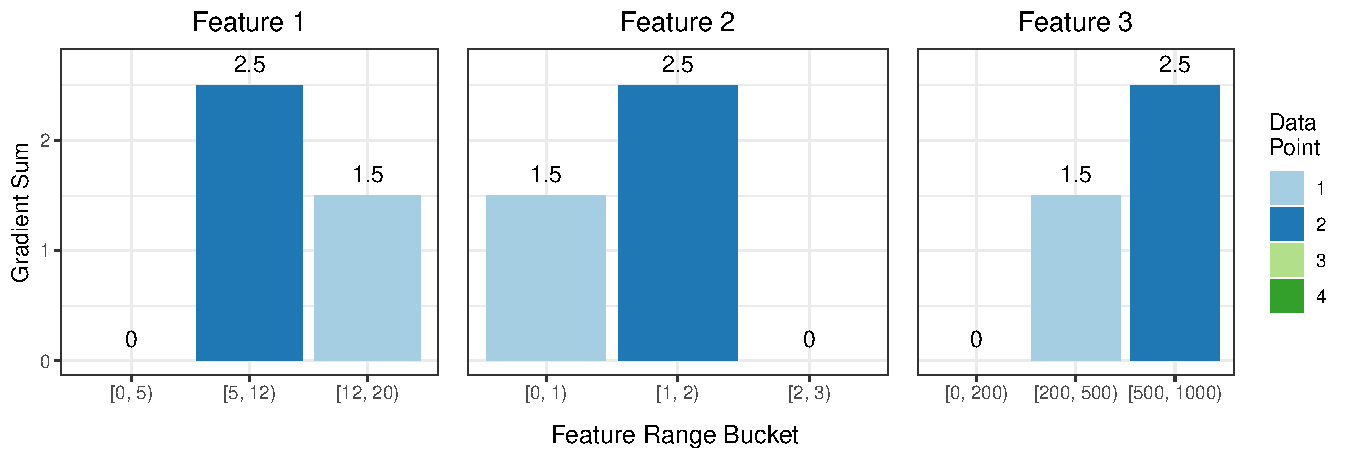
\includegraphics[width=\linewidth]{all-features-grad-rowdist-w1}
		\caption{Local gradient histogram for Worker 1.}
		\label{fig:grad-row-dist-w1}
	\end{subfigure}
	\\
	\begin{subfigure}[t]{\textwidth}
		\centering
		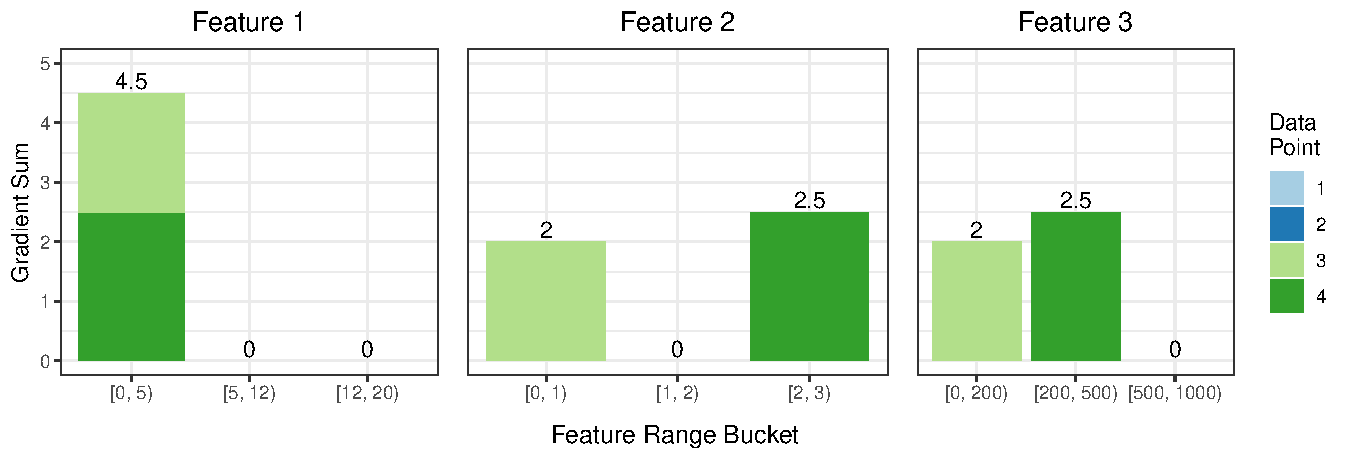
\includegraphics[width=\linewidth]{all-features-grad-rowdist-w2}
		\caption{Local gradient histogram for Worker 2.}
		\label{fig:grad-row-dist-w2}
	\end{subfigure}
	\caption{Local gradient histograms for row-distributed data. Note the existence of multiple
	zero values that would nonetheless need to be communicated using a dense communication pattern like
	MPI allreduce.}
	\label{fig:grad-row-dist}
\end{figure}


One drawback of all current row-distributed methods is that they use dense communication
for the aggregation we just described~\cite{xgboost, lightgbm, catboost, dimboost}. Dense communication
requires us to communicate $|F| \cdot B$ values for each worker, where $F$ the set of features,
and $B$ the number of histogram buckets. However,
many of the histogram values can be zero as can be seen in Figure \ref{fig:grad-row-dist}, where we show
the local gradient histograms for each worker. This results in redundant communication when
a dense communication pattern is used. This problem is exacerbated when we are dealing with sparse
datasets with millions of features.

Block-distribution introduces another level of complexity into this operation, as
in that case, no worker has a complete view of any data point. Each worker gets one block,
that is, a horizontal \emph{and} vertical slice of the data. If we think of the complete
gradient histograms as a tensor of dimensions $|L| \times |F| \times B$, each worker
will populate a part of this tensor, across the $L$ (leafs) and $B$ (buckets) dimensions, but limited to a specific
subset of $F$ (features). In \blockgbt, we use a sparse representation of this tensor at each worker
which we then send to the servers, which allows
us to eliminate the extraneous communication described above. Our experiments show
that for sparse datasets this brings the communication cost down by multiple orders
of magnitude.

Once each worker iterates
through their block of data, they send their partial tensor to one server. Each server
is now responsible for a range of features, so workers that belong to the same \emph{vertical}
slice of data will send their tensors to the same server. Each server ends up having
a full view of the gradient histograms for a subset of features. The split finding step
can then be performed using an algorithm similar to the one proposed in \citet{dimboost}.

\section{Main Findings}

In this section we present the evaluation of the online distributed tree boosting
algorithm from \boostvht and the block-distributed GBT algorithm from \blockgbt.

\subsubsection*{Online and Distributed Boosted Trees}
\label{sec:boostvht-results}

For our online learning experiments of BoostVHT we use 10 artificial and 4 real-world datasets. The artificial
datasets are generated with different numbers of attributes using one generator
from a tree-like structure, one that generates random tweet text for a sentiment
analysis task, and one rotating hyperplane. The baselines we test against are
a single-threaded online boosting algorithm from the MOA \cite{bifet2010moa}
library using the Hoeffding tree as a base learner, and the base VHT tree.
We measure the speedup over the single-threaded algorithm, and use the
robust Kappa~\cite{bifet2015efficient} statistic to measure accuracy,
that considers the probability of agreement by chance in the evaluation.

We start by showing that the boosted version of the algorithm performs
better than the base VHT. Figure \ref{fig:boostvht-textgen-accuracy} shows an example experiment using different
levels of dimensionality for the text-generator data. We can see
that as we increase the number of features and make the problem more
difficult, the accuracy of the VHT algorithm deteriorates, while
BoostVHT is consistently accurate, and is practically equivalent to the single-threaded
boosting algorithm. At the same time, the concurrent and parallel design of the algorithm
provides us with a speedup of \textbf{$\times$45} on average, compared to the single-threaded
implementation of MOA (shown in Table 2 of \boostvht).

\begin{figure*}
	\centering
	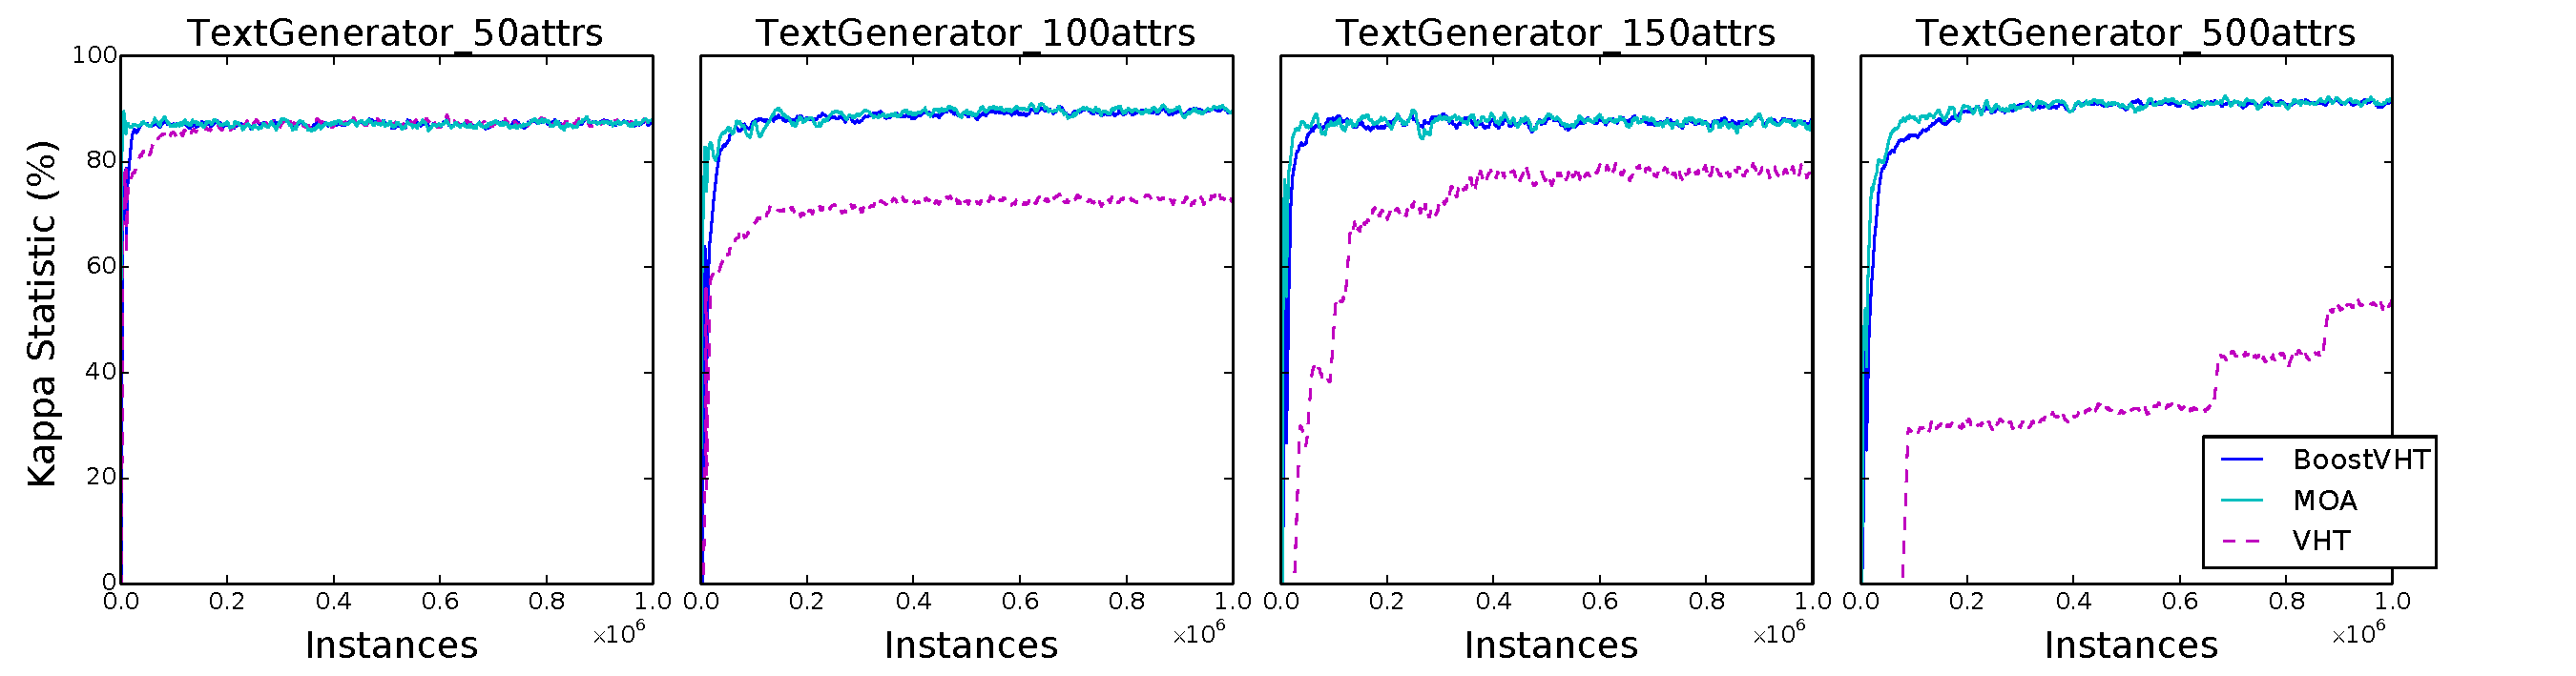
\includegraphics[width=\textwidth]{textGen_all_kappa_stat_storm.pdf}
	\caption{Kappa statistic (accuracy) as a function of arriving instances over time for text generator datasets with
		an increasing number of attributes.}
	\label{fig:boostvht-textgen-accuracy}
\end{figure*}

Finally we examine the scalability of the algorithm in terms of strong and weak scaling.
Ideal strong scaling provides \emph{linear speed-up}: Doubling the amount of resources
while keeping the problem size constant should halve the execution time.
Ideal weak scaling should have \emph{linear scale-out}: doubling both the problem size
and resources at the same time should not affect the training time significantly.
We illustrate the scaling characteristics of the algorithm in Figures
\ref{fig:weak-scaling} and \ref{fig:strong-scaling} for weak and strong
scaling respectively. As we can see in the figures, the algorithm scales
almost ideally both in terms of weak scaling, keeping its training time
close to constant as we double resources and the problem size, and provides
near-linear speed-up for our strong scaling experiments.

\begin{figure}
	\centering
	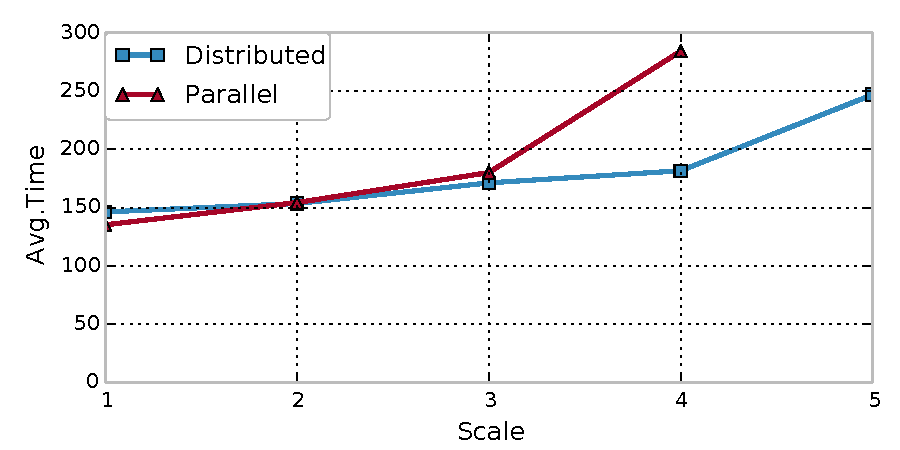
\includegraphics[width=0.8\textwidth]{weak-scaling.pdf}
	\caption{Weak scaling experiments, time in milliseconds. Scale 1x on the x-axis refers to 500 attributes with 2 Processors, and we double both Processors and attributes for each scale increment (up to 8,000 attributes with 32 Processors).}
	\label{fig:weak-scaling}
\end{figure}

\begin{figure}
	\centering
	\begin{subfigure}[t]{0.5\textwidth}
		\centering
		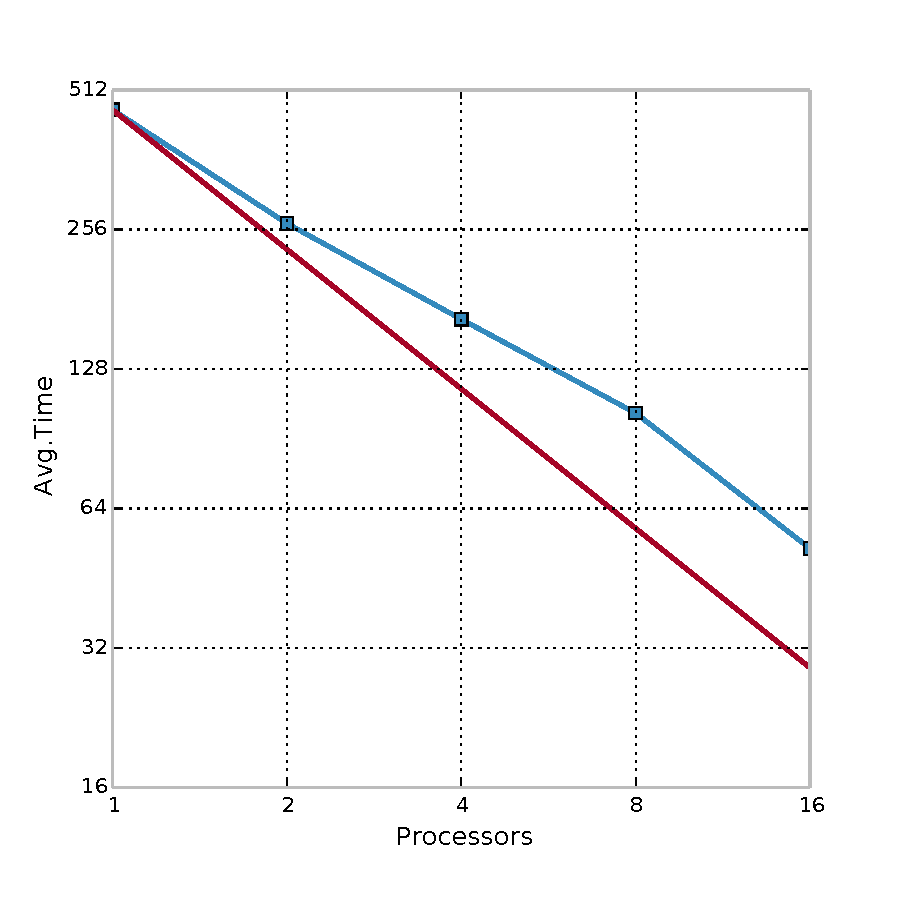
\includegraphics[width=\linewidth]{ice-strong-scaling.pdf}
		\caption{Parallel experiments.}
		\label{fig:strong-parallel}
	\end{subfigure}%
	\begin{subfigure}[t]{0.5\textwidth}
		\centering
		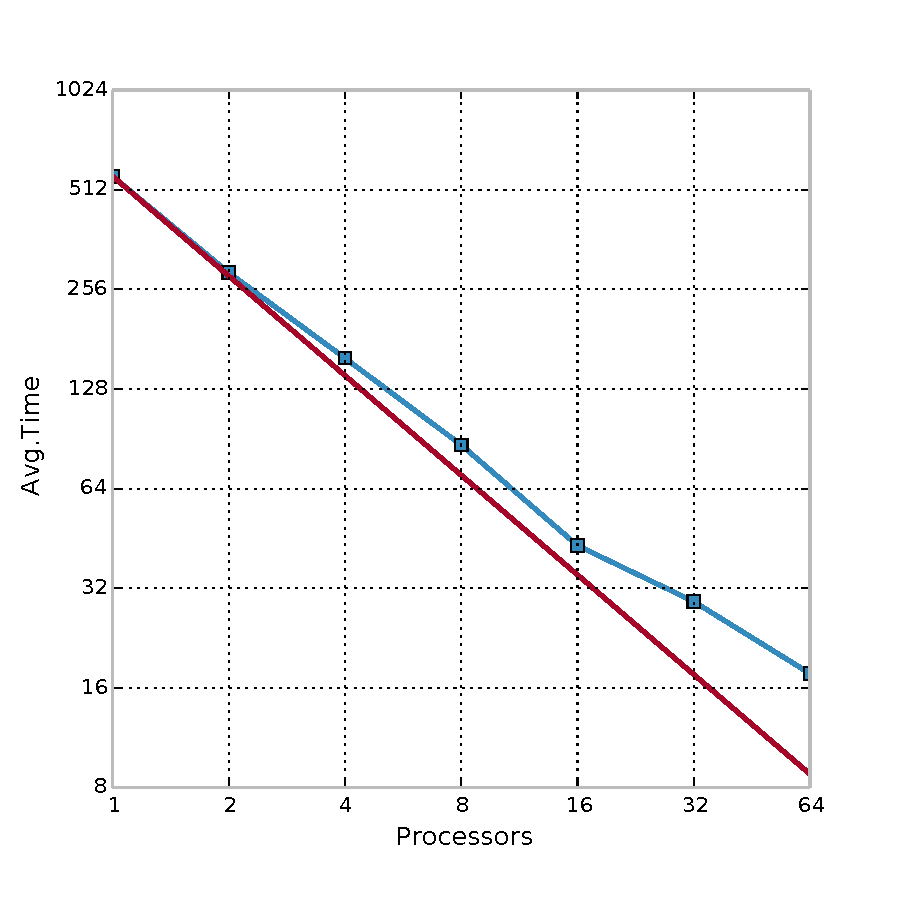
\includegraphics[width=\linewidth]{ec2-strong-scaling.pdf}
		\caption{Distributed experiments}
		\label{fig:strong-distributed}
	\end{subfigure}
	\caption{Strong scaling in the parallel (left) and distributed (right) setting. The
		time reported is the average time to train 1,000 instances, each with 1,000 attributes, in milliseconds. The red straight line indicates ideal linear scaling.}
	\label{fig:strong-scaling}
\end{figure}

\subsubsection*{Block-distributed Gradient Boosted Trees}
\label{sec:block-gbt-results}

To determine the performance gains and limitations of our block-distributed approach and
the sparse communication we employ, over the dense row-distributed approach,
we use 4 datasets with different sparsity levels. First
we have two highly sparse datasets, URL and avazu with roughly 3,2 million and
1 million features respectively. Second, we use the RCV1 dataset with approximately
47 thousand features and the dense Bosch dataset with 968 features.
We implement both approaches from scratch in C++ to ensure a fair comparison.
We use 12 workers for the row-distributed approach, and 9 workers and 3
servers for the block-distributed approach.

We measure the
communication cost in MiB for the dense histograms of the row-distributed approach
and our sparse block-distributed histograms. We also evaluate the end-to-end runtime
of the histogram aggregation step, divided into communication and computation stages,
to measure the real-world runtime. This step is the most computationally intensive
part of GBT learning \cite{comm-efficient-gbt} and in our experiments constitutes
at least 90\% of the total runtime of the training.

In Figure \ref{fig:block-gbt-hist-size} we can see the benefits of sparse communication:
For the highly sparse URL and avazu datasets the reduction in communication is five and
two orders of magnitude respectively. The sparse histograms however introduce additional computational
cost: unlike dense data structures that are contiguous in memory, sparse structures use
indirect addressing which makes building and accessing these histograms cache-unfriendly.
This, in combination with the overhead introduced by the use of the parameter server,
leads to increased computation time.
While in the sparse datasets the significant gains made by minimizing the communication time
allows us to compensate for the increased computation, that is not the case for
the dense data, where computation time dominates, as shown in Figure \ref{fig:block-gbt-time}.


\begin{figure}
	\centering
	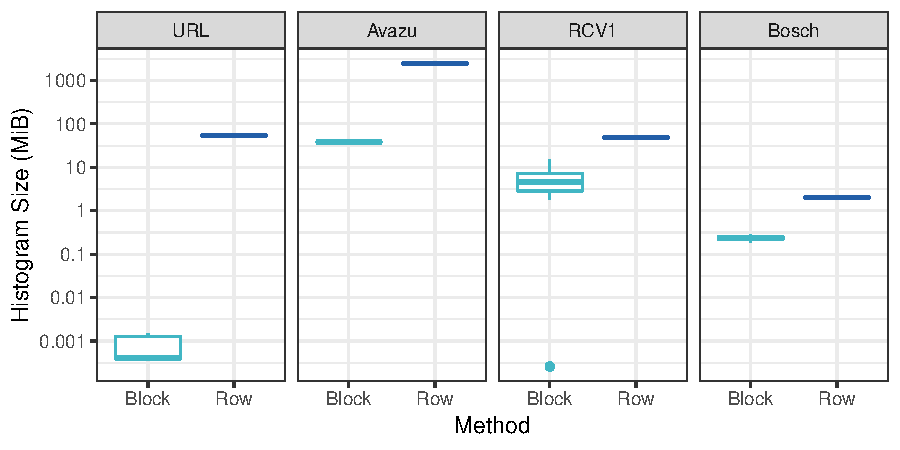
\includegraphics[width=0.8\textwidth]{block-gbt-hist-box.pdf}
	\vspace{-10pt}
	\caption{The byte size of the gradient histograms being communicated for the various datasets.}
	\label{fig:block-gbt-hist-size}
\end{figure}

\begin{figure}
	\centering
	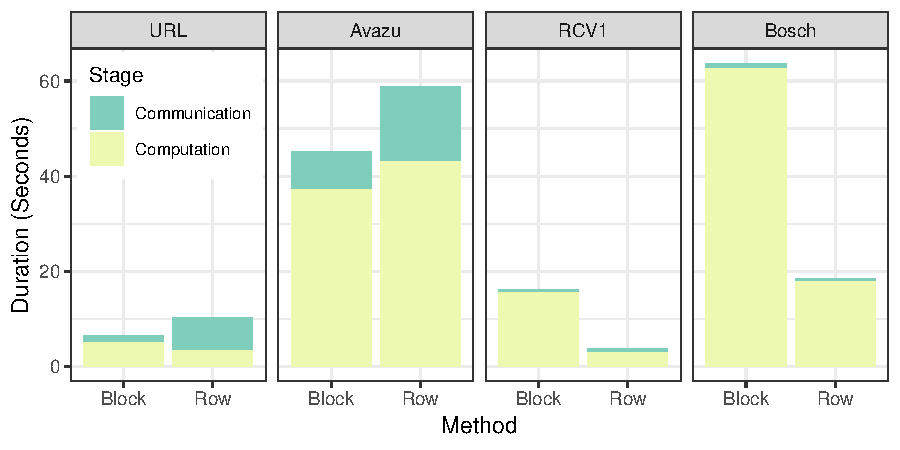
\includegraphics[width=0.8\textwidth]{block-gbt-time.pdf}
	\vspace{-10pt}
	\caption{The communication and computation times for the various datasets, in seconds.}
	\label{fig:block-gbt-time}
\end{figure}


Finally we demonstrate the communication savings possible in terms of the feature sketches.
As we mentioned in Section \ref{sec:bg-dt-gbts}, in order to determine the possible
split points for each feature, we need to have an estimate of the CDF for each feature. These
can be calculated once at the beginning of learning, or once per leaf, to get a more accurate representation
of the CDF in every leaf. \citet{xgboost} show that generating per-leaf (local) split points leads to the same overall
accuracy as using the overall sketches (global) while using much less accurate sketches, thereby creating potential communication savings:
The size of a quantile sketch is determined by the level of error in the approximation we can
accept~\cite{karnin2016kll}, and the values we populate it with.

However, when using dense communication we need to know the size
of the sketch being communicated in advance. In a probabilistic sketch, this is only possible
if we use the maximum theoretical size of a sketch, to ensure the sketches do not overlap in memory.
This of course is a major source of inefficiency, as the actual size of the sketches can be orders
of magnitude smaller. For this reason
current distributed approaches all use the global sketch approach, in order to only communicate
the sketches once at the beginning of learning instead of having to communicate once for every
leaf.

Using our sparse approach however, allows us to only communicate the true size of the sketches,
thereby providing massive savings in communication, as shown in Figure \ref{fig:block-gbt-sketch-size}. This would allow the sketches to be communicated for every
leaf, leading to even further savings by using lower accuracy sketches or increased accuracy
in the CDF representation.

\begin{figure}
	\centering
	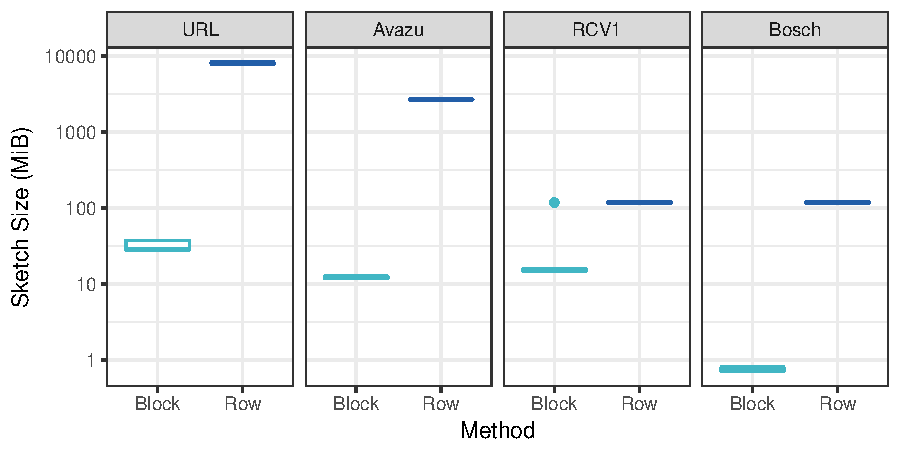
\includegraphics[width=0.8\textwidth]{block-gbt-sketch-box.pdf}
	\vspace{-10pt}
	\caption{The byte size of the feature sketches being communicated for the various datasets.}
	\label{fig:block-gbt-sketch-size}
\end{figure}

\section{Discussion}

In this chapter we have presented our work on scalable boosted
trees. We first developed a model-parallel online algorithm with linear scaling
characteristics and demonstrated its accuracy advantages over single
trees and significant runtime gains compared to serial tree ensembles.
We have used efficient communication to dramatically reduce the number
of messages sent.

Second, we developed a block-distributed gradient boosted tree
algorithm. Apart from enabling scale-out across both the feature
and data point dimensions, we took advantage of data sparsity
to reduce the communication necessary for training by several
orders of magnitude.

Thus, these studies demonstrated how
algorithmic co-design with distributed systems can lead
to optimized runtimes and communication savings, aligning
this work with our objectives and research question
defined in Section \ref{sec:intro-question-objectives}.
We note however that the benefit of both approaches
is limited when the dimensionality of the data is low.